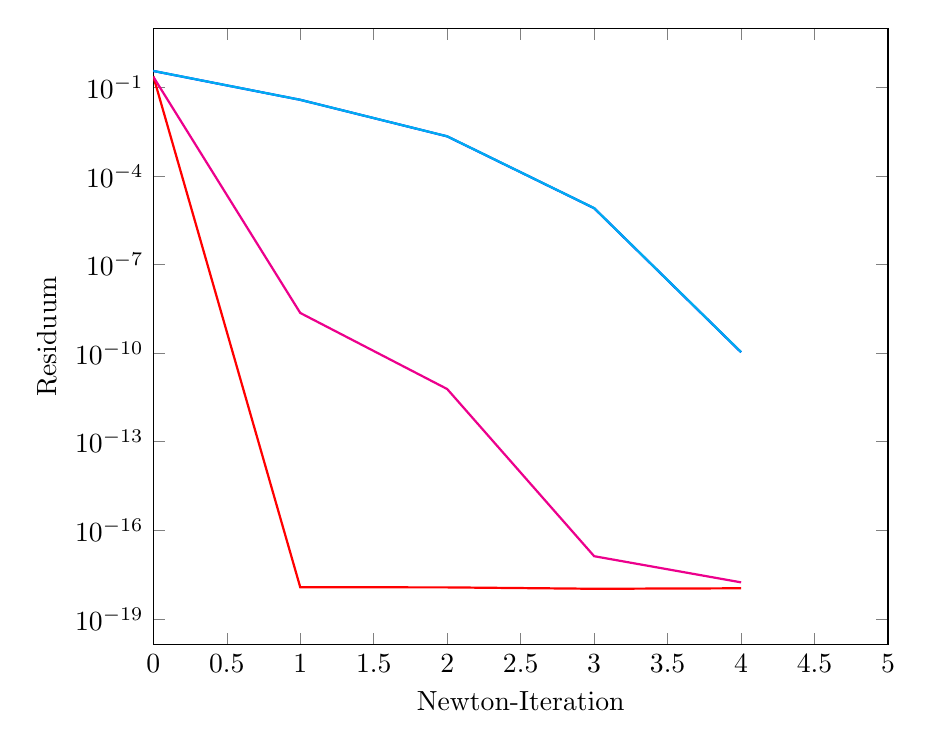
\begin{tikzpicture}[every plot/.append style={thick}] 
\begin{axis}[ 
label style={font=\normalsize}, 
xlabel={Newton-Iteration}, 
ylabel={Residuum}, 
xmin=0, xmax=5, 
ymode=log, 
ymin=0, ymax=10, 
width=0.9\textwidth, 
grid style=dashed, 
] 
\addplot[ 
color=blue, 
] 
coordinates { 
(0, 3.57e-01)(1, 3.77e-02)(2, 2.18e-03)(3, 8.07e-06)(4, 1.07e-10)}; 
\addplot[ 
color=red, 
] 
coordinates { 
(0, 2.37e-01)(1, 1.18e-18)(2, 1.17e-18)(3, 1.05e-18)(4, 1.09e-18)}; 
\addplot[ 
color=cyan, 
] 
coordinates { 
(0, 3.59e-01)(1, 3.77e-02)(2, 2.19e-03)(3, 8.11e-06)(4, 1.08e-10)}; 
\addplot[ 
color=magenta, 
] 
coordinates { 
(0, 2.27e-01)(1, 2.29e-09)(2, 6.08e-12)(3, 1.33e-17)(4, 1.73e-18)}; 
\end{axis} 
\end{tikzpicture} 
